\documentclass{article}

% to compile a camera-ready version, add the [final] option, e.g.:
    \usepackage[final]{neurips_2023}
    
\usepackage[utf8]{inputenc} % allow utf-8 input
\usepackage[T1]{fontenc}    % use 8-bit T1 fonts
\usepackage{hyperref}       % hyperlinks
\usepackage{url}            % simple URL typesetting
\usepackage{booktabs}       % professional-quality tables
\usepackage{amsfonts}       % blackboard math symbols
\usepackage{nicefrac}       % compact symbols for 1/2, etc.
\usepackage{microtype}      % microtypography
\usepackage{xcolor}         % colors
\usepackage{graphicx}
\usepackage{amsmath}
\usepackage{float}

\title{AlphaDou: \\ Multi-Agent Search and Learning for Jungle Chess}


\author{%
  Zihan Wang \\
  \texttt{wangzh12023} \\
  \And
  Ziyu Cheng \\
  \texttt{chengzy2023} \\
  \And
  Mingfei Xia \\
  \texttt{xiamf2023} \\
}

\begin{document}


\maketitle


\begin{abstract}
In a simplified Jungle Chess environment ($7\times8$ board, omitting traps, rivers, and dens), we implemented and compared seven agents: Random, Greedy (heuristic), Minimax, Tabular Q-Learning, Approximate Q‐Learning and Deep Q-Network (DQN). Each agent was evaluated via self-play and round-robin tournaments, comparing win rates and decision-making latency. We also conducted ablation studies to assess the impact of heuristic weights and the discount factor on learning performance. Our results demonstrate the applicability of various search and learning methods to Jungle Chess and provide a foundation for future reinforcement learning research incorporating neural priors or full game rules.
\end{abstract}


\section{Introduction}

\subsection{Game Settings}

\begin{itemize}
    \item \textbf{Board}: $7 \times 8$ Grid
    \item \textbf{Pieces}: 8 pieces per side: Elephant (Rank 8), Lion (Rank 7), Tiger (Rank 6), Leopard (Rank 5), Wolf (Rank 4), Dog (Rank 3), Cat (Rank 2), Rat (Rank 1)
    \item \textbf{Simplified Rules}:
    \begin{itemize}
        \item Rank‐based Predation: A piece of higher rank can capture (eat) any opposing piece of strictly lower rank. But a Rat (Rank 1) can capture an Elephant (Rank 8)
        \item No Traps / No Rivers / No Dens:
        
        \item Action: Each turn, a player must either move  one revealed piece to an adjacent (up/down/left/right) empty square or reveal one  face‐down pieces if any remain.
    
        \item Game End Condition:
        \begin{itemize}
            \item Win by Elimination: A player who captures all of the opponent’s remaining pieces immediately wins.
            \item Stalemate Rule: If no capture occurs in 100 consecutive moves (both sides combined), the game is declared a draw.
        \end{itemize}
    \end{itemize}
\end{itemize}

\begin{figure}
    \centering
    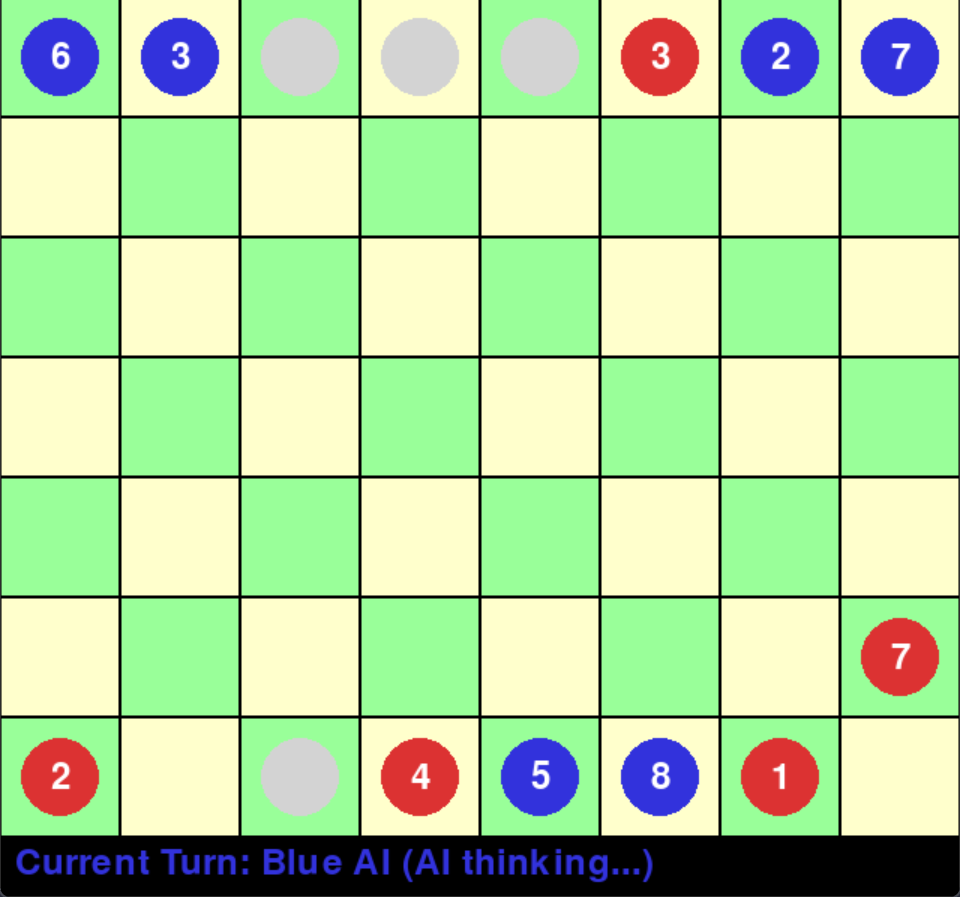
\includegraphics[width=0.3\textwidth]{UISHOW.png}
    \caption{Visulization of Jungle Chess game board}
    \label{fig:confusion}
\end{figure}
\subsection{State Space}

\subsubsection{State Representation}
\begin{itemize}
    \item A \emph{state} is fully determined by the set of all remaining pieces and their board positions.
    \item In our simplified rules, there are no traps, rivers, or dens, so all 16 pieces (8 per side) occupy one of the 56 squares.
    \item We encode a state as an ordered tuple of 16 triples:
    \[
      s \;=\;\bigl((p_1,x_1,y_1),\, (p_2,x_2,y_2),\,\dots,\,(p_{16},x_{16},y_{16})\bigr),
    \]
    where:
    \begin{itemize}
      \item \(p_i \in \{\text{Black Elephant},\,\dots,\,\text{White Rat}\}\) specifies piece identity (type and color), and
      \item \((x_i,y_i)\) is the square coordinate (row and column) of that piece.
    \end{itemize}
    \item Once two pieces occupy the same square, the lower‐rank piece is captured (removed), so no square holds more than one piece.
\end{itemize}

\subsubsection{Combinatorial Size}
\begin{itemize}
    \item There are 56 total squares and 16 distinct pieces.
    \item To place 16 Black pieces on 56 squares and order matters: $\binom{56}{16} \times 16!$
    \item And every piece has two states: revealed or unrevealed: $\binom{56}{16} \times 16! \times 2^{16}$
    \item And two people's turn counts as two different situations: $\binom{56}{16} \times 16! \times 2^{16} \times 2$
    \[
      \bigl|\mathcal{S}\bigr|
      \;=\;\binom{56}{16} \times 16! \times 2^{16} \times 2 \approx 2^{32}
    \]
\end{itemize}

%%%%%%%%%%%%%%%%%%%%%%ToDO%%%%%%%%%%%%%%%%%%%%%%%%%%%%%%%%%%%%
%%%%%%%%%%%%%%%%%%%%%%ToDO%%%%%%%%%%%%%%%%%%%%%%%%%%%%%%%%%%%%
%%%%%%%%%%%%%%%%%%%%%%ToDO%%%%%%%%%%%%%%%%%%%%%%%%%%%%%%%%%%%%
%%%%%%%%%%%%%%%%%%%%%%ToDO%%%%%%%%%%%%%%%%%%%%%%%%%%%%%%%%%%%%
\subsubsection{Action Space}
\begin{itemize}
    \item In any given state \(s\), a player’s legal actions consist of:
    \begin{itemize}
      \item Moving one revealed piece to an adjacent empty square (up, down, left, or right), provided it does not violate rank‐based capture rules.
      \item Flipping (revealing) one of their own face‐down pieces, if any remain.
    \end{itemize}
    \item Each revealed piece can have up to 4 orthogonal moves, subject to:
    \begin{itemize}
      \item The destination square must be empty or occupied by an opponent’s piece of strictly lower rank (with the Rat–Elephant exception).
      \item No diagonal moves are allowed.
    \end{itemize}
\end{itemize}


\section{Methods}


\subsection{RandomAgent}
The Random Agent implements the simplest decision-making strategy in our Chinese Dark Chess system. It serves as a baseline player that makes completely random moves without any strategic consideration or game state evaluation.
The Random Agent follows this simple procedure:
\begin{enumerate}
    \item \textbf{Action Retrieval}: Obtains all possible legal actions from the current board state.
    \item \textbf{Randomization}: Shuffles the list of possible actions using.
    \item \textbf{Action Execution}: Iterates through the shuffled actions and attempts to execute the first valid one:
\end{enumerate}

\subsection{GreedyAgent}

The Greedy Agent implements a heuristic-based decision-making strategy that evaluates all possible moves and selects the action that provides the highest immediate score improvement. Unlike the Random Agent, it incorporates strategic thinking through a comprehensive evaluation function, but without lookahead planning like more sophisticated algorithms.

The GreedyPlayer class uses a multi-component evaluation function based on the comprehensive formula:
$$\text{Score}(s) = \sum_{i=1}^{4} \text{Component}_i(s)$$

Where the components and parameters are defined as follows:
\begin{enumerate}
    \item   \textbf{Piece Value Component:}
            \\
            \\
            This component evaluates the material advantage of the agent.
            \begin{equation}
                \label{eq:piece_value}
                \text{Component}_1(s) = \sum_{p \in P_{\text{self}}} V(p) - \lambda_1 \sum_{p \in P_{\text{opp}}} V(p)
            \end{equation}
            Here:
            \begin{itemize}
                \item $P_{\text{self}}$ and $P_{\text{opp}}$ are the sets of pieces belonging to the self and the opponent respectively.
                \item $V(p)$ is the value function for a piece $p$:
                \begin{equation}
                \label{eq:piece_value_function}
                V(p) = \begin{cases}
                \textit{piece\_values}[\text{strength}(p)] & \text{if } p.\text{revealed} = \text{True} \\
                V_{\text{unrevealed}} & \text{if } p.\text{revealed} = \text{False}
                \end{cases}
                \end{equation}
                \item $\textit{piece\_values}$ is a mapping from piece strength to its intrinsic value:
                \begin{align*}
                    \textit{piece\_values} = \{& 8 \mapsto 80, \quad 7 \mapsto 70, \quad 6 \mapsto 60, \quad 5 \mapsto 50, \\
                    & 4 \mapsto 40, \quad 3 \mapsto 30, \quad 2 \mapsto 20, \quad 1 \mapsto 30 \}
                \end{align*}
                \item $V_{\text{unrevealed}} = 30$ is the estimated value for an unrevealed piece.
                \item $\lambda_1 = 0.8$ is the opponent piece weight coefficient.
            \end{itemize}
            

    \item   \textbf{Positional Reward Component:}
            \\
            \\
            This component rewards pieces for occupying advantageous board positions.
            \begin{equation}
                \label{eq:positional_reward}
                \text{Component}_2(s) = \lambda_3' \sum_{p \in P_{\text{self}}^{\text{revealed}}} \left( f_{\text{advance}}(p) + f_{\text{center}}(p) \right)
            \end{equation}
            Here:
            \begin{itemize}
                \item $P_{\text{self}}^{\text{revealed}}$ is the set of revealed pieces belonging to the agent.
                \item $f_{\text{advance}}(p)$ is the advance reward function for piece $p$:
                \begin{equation}
                \label{eq:advance_reward}
                f_{\text{advance}}(p) = \begin{cases}
                5 \times \text{row}(p) & \text{if player\_id} = 0 \\
                5 \times (\text{ROWS} - 1 - \text{row}(p)) & \text{if player\_id} = 1
                \end{cases}
                \end{equation}
                where $\text{row}(p)$ is the row index of piece $p$, $\text{ROWS}$ is the total number of rows on the board, and $\text{player\_id}$ identifies the current player.
                \item $f_{\text{center}}(p)$ is the central control reward function for piece $p$:
                \begin{equation}
                \label{eq:center_reward}
                f_{\text{center}}(p) = \begin{cases}
                5 & \text{if col}(p) \in \{\lfloor \text{COLS}/2 \rfloor - 1, \lfloor \text{COLS}/2 \rfloor\} \\
                0 & \text{otherwise}
                \end{cases}
                \end{equation}
                where $\text{col}(p)$ is the column index of piece $p$, and $\text{COLS}$ is the total number of columns on the board.
                \item $\lambda_3' = \frac{\lambda_3}{10} = \frac{15}{10} = 1.5$ is the scaled positional weight coefficient. (Original $\lambda_3 = 15$).
            \end{itemize}

            
            
    \item  \textbf{Mobility Component:}
            \\
            \\
            This component rewards the agent for having a larger number of available moves.
            \begin{equation}
                \label{eq:mobility}
                \text{Component}_3(s) = \lambda_2 |A_{\text{possible}}(s)|
            \end{equation}

            
            Here:
            \begin{itemize}
                \item $A_{\text{possible}}(s)$ is the set of all legal actions available to the agent in state $s$.
                \item $|A_{\text{possible}}(s)|$ denotes the number of possible actions.
                \item $\lambda_2 = 2$ is the mobility weight coefficient.
            \end{itemize}
            
    \item  \textbf{Mobility Component:}
            \\
            \\
            This component evaluates the immediate threats and advantages in engagements between adjacent pieces.

            
            \begin{equation}
                \label{eq:safety}
                \text{Component}_4(s) = w_{\text{safety}} \sum_{p_s \in P_{\text{self}}^{\text{revealed}}} \sum_{p_o \in P_{\text{opp}}^{\text{revealed}}} \text{ThreatValue}(p_s, p_o)
            \end{equation}
            Here:
            \begin{itemize}
                \item $P_{\text{self}}^{\text{revealed}}$ and $P_{\text{opp}}^{\text{revealed}}$ are the sets of revealed pieces for the agent and opponent, respectively.
                \item $\text{ThreatValue}(p_s, p_o)$ is the function evaluating the threat between an agent's piece $p_s$ and an opponent's piece $p_o$:
                \begin{equation}
                \label{eq:threat_value}
                \text{ThreatValue}(p_s, p_o) = \begin{cases}
                -10 & \text{if } \text{Adjacent}(p_s, p_o) \land \text{CanCapture}(p_o, p_s) \\
                +15 & \text{if } \text{Adjacent}(p_s, p_o) \land \text{CanCapture}(p_s, p_o) \\
                0 & \text{otherwise}
                \end{cases}
                \end{equation}
                \item $\text{Adjacent}(p_1, p_2)$ is a boolean function that returns true if pieces $p_1$ and $p_2$ are adjacent on the board.
                \item $\text{CanCapture}(p_1, p_2)$ is a boolean function determining if piece $p_1$ can capture piece $p_2$:
                \begin{equation}
                \label{eq:can_capture}
                \text{CanCapture}(p_1, p_2) = \begin{cases}
                \text{True} & \text{if } (\text{strength}(p_1) > \text{strength}(p_2)) \\ & \quad \land \neg(\text{strength}(p_1) = 8 \land \text{strength}(p_2) = 1) \\
                \text{True} & \text{if } \text{strength}(p_1) = 1 \land \text{strength}(p_2) = 8 \\
                \text{False} & \text{otherwise}
                \end{cases}
                \end{equation}
                where $\text{strength}(p)$ denotes the strength of piece $p$.
                \item $w_{\text{safety}} = 10$ is the safety weight coefficient.
            \end{itemize}
            
    
\end{enumerate}

The overall heuristic $H(s)$ combines these components using their respective weights: $\lambda_1=0.8$, $\lambda_2=2$, $\lambda_3'=1.5$, and $w_{\text{safety}}=10$.

The heuristic evaluation function, $H(s)$, for the GreedyAgent is a weighted sum of four components: piece value, positional reward, mobility, and safety. The state of the game is denoted by $s$.

\begin{equation}
\label{eq:total_heuristic}
\begin{split}
H(s) = & \left( \sum_{p \in P_{\text{self}}} V(p) - \lambda_1 \sum_{p \in P_{\text{opp}}} V(p) \right) \\
& + \lambda_3' \sum_{p \in P_{\text{self}}^{\text{revealed}}} \left( f_{\text{advance}}(p) + f_{\text{center}}(p) \right) \\
& + \lambda_2 |A_{\text{possible}}(s)| \\
& + w_{\text{safety}} \sum_{p_s \in P_{\text{self}}^{\text{revealed}}} \sum_{p_o \in P_{\text{opp}}^{\text{revealed}}} \text{ThreatValue}(p_s, p_o)
\end{split}
\end{equation}




\subsection{MinimaxAgent}
The evaluation function for the MinimaxAgent, denoted as $H_{\text{minimax}}(s)$, assesses the desirability of a game state $s$. It is composed of four distinct components, each contributing to the overall score.

The complete Minimax evaluation function is defined as:
\begin{equation}
\label{eq:minimax_total_heuristic}
\begin{split}
H_{\text{minimax}}(s) = w_1 & (|P_{\text{self}}| - |P_{\text{opp}}|) \\
& + w_2 \left(\sum_{p \in P_{\text{self}}^{\text{revealed}}} \text{strength}(p) - \sum_{p \in P_{\text{opp}}^{\text{revealed}}} \text{strength}(p)\right) \\
& + \left( w_{3a} |P_{\text{self}}^{\text{unrevealed}}| - w_{3b} |P_{\text{opp}}^{\text{unrevealed}}| \right) \\
& + \sum_{p_s \in P_{\text{self}}^{\text{revealed}}} \sum_{p_o \in P_{\text{opp}}^{\text{revealed}}} \text{TacticalValue}(p_s, p_o)
\end{split}
\end{equation}
where the specific weights and components are detailed below:

\begin{enumerate}
    \item \textbf{Piece Count Difference Component}
            \\
            \\
            This component measures the raw numerical advantage in pieces.
            \begin{equation}
            \label{eq:minimax_c1_base}
            C_1(s) = w_1 (|P_{\text{self}}| - |P_{\text{opp}}|)
            \end{equation}
            Where:
            \begin{itemize}
                \item $|P_{\text{self}}|$ is the total number of pieces for the agent (self).
                \item $|P_{\text{opp}}|$ is the total number of pieces for the opponent.
                \item  $w_1 = 1$.
            \end{itemize}
    
    \item  \textbf{Piece Strength Sum Component}
            \\
            \\
            This component evaluates the difference in the sum of strengths of revealed pieces.
            \begin{equation}
            \label{eq:minimax_c2_base}
            C_2(s) = w_2 \left(\sum_{p \in P_{\text{self}}^{\text{revealed}}} \text{strength}(p) - \sum_{p \in P_{\text{opp}}^{\text{revealed}}} \text{strength}(p)\right)
            \end{equation}
            Where:
            \begin{itemize}
                \item $P_{\text{self}}^{\text{revealed}}$ and $P_{\text{opp}}^{\text{revealed}}$ are the sets of revealed pieces for the self and opponent respectively.
                \item $\text{strength}(p) \in \{1, 2, 3, 4, 5, 6, 7, 8\}$ denotes the strength of piece $p$.
                \item $w_2 = 10$
            \end{itemize}
            

            
    \item  \textbf{Information Value Component}
            \\
            \\
            This component quantifies the value of information asymmetry based on unrevealed pieces.
            \begin{equation}
            \label{eq:minimax_c3}
            C_3(s) = w_{3a} |P_{\text{self}}^{\text{unrevealed}}| - w_{3b} |P_{\text{opp}}^{\text{unrevealed}}|
            \end{equation}
            Where:
            \begin{itemize}
                \item $P_{\text{self}}^{\text{unrevealed}}$ and $P_{\text{opp}}^{\text{unrevealed}}$ are the sets of unrevealed pieces for the agent and opponent, respectively.
                \item $w_{3a} = 5$ is the value assigned to each of the agent's unrevealed pieces (potential resources).
                \item $w_{3b} = 10$ is the negative value assigned to each of the opponent's unrevealed pieces (unknown threats).
            \end{itemize}
            This component is used directly in $H_{\text{minimax}}(s)$ as defined.
            
    \item  \textbf{Threat Opportunity Component}
            \\
            \\
            This component  assesses immediate tactical threats and opportunities between adjacent revealed pieces.
            \begin{equation}
            \label{eq:minimax_c4}
            C_4(s) = \sum_{p_s \in P_{\text{self}}^{\text{revealed}}} \sum_{p_o \in P_{\text{opp}}^{\text{revealed}}} \text{TacticalValue}(p_s, p_o)
            \end{equation}
            Where:
            \begin{itemize}
                \item $p_s$ is a revealed piece belonging to the agent, and $p_o$ is a revealed piece belonging to the opponent.
                \item $\text{TacticalValue}(p_s, p_o)$ is the function evaluating the tactical situation:
                \begin{equation}
                \label{eq:minimax_tactical_value}
                \text{TacticalValue}(p_s, p_o) = \begin{cases}
                +20 & \text{if } \text{Adjacent}(p_s, p_o) \land \text{CanCapture}(p_s, p_o) \\
                -15 & \text{if } \text{Adjacent}(p_s, p_o) \land \text{CanCapture}(p_o, p_s) \\
                0 & \text{otherwise}
                \end{cases}
                \end{equation}
                \item $\text{Adjacent}(p_1, p_2)$ is a boolean function, true if pieces $p_1$ and $p_2$ are adjacent.
                \item $\text{CanCapture}(p_1, p_2)$ is a boolean function indicating if $p_1$ can capture $p_2$ 
            \end{itemize}
            
            
            
\end{enumerate}





\subsection{Q-Learning}

\subsubsection{Basic State Definition}
The state tensor $\mathbf{S} \in \mathbb{R}^{7 \times 8 \times 4}$ is defined where each position $(r,c)$ has a feature vector:
$$ \mathbf{s}_{r,c} = \begin{bmatrix}
p_{r,c} \\
\frac{\text{strength}_{r,c}}{8} \\
\mathbb{I}_{\text{revealed}}(r,c) \\
\mathbb{I}_{\text{occupied}}(r,c)
\end{bmatrix} \in \mathbb{R}^4 $$

Where:
$$ p_{r,c} = \begin{cases}
0 & \text{if piece at }(r,c)\text{ belongs to player 0} \\
1 & \text{if piece at }(r,c)\text{ belongs to player 1} \\
0 & \text{if position }(r,c)\text{ is empty}
\end{cases} $$

$$ \frac{\text{strength}_{r,c}}{8} = \begin{cases}
\frac{k}{8} & \text{if piece at }(r,c)\text{ has strength }k \in \{1,2,\ldots,8\} \\
0 & \text{if position }(r,c)\text{ is empty}
\end{cases} $$

$$ \mathbb{I}_{\text{revealed}}(r,c) = \begin{cases}
1 & \text{if piece at }(r,c)\text{ is revealed} \\
0 & \text{otherwise}
\end{cases} $$

$$ \mathbb{I}_{\text{occupied}}(r,c) = \begin{cases}
1 & \text{if position }(r,c)\text{ contains a piece} \\
0 & \text{if position }(r,c)\text{ is empty}
\end{cases} $$

And the \textbf{Action Space} is defined as
\begin{itemize}
    \item \textbf{Reveal Action}: $(\text{"reveal", (row, col)})$ for unrevealed own pieces
    \item \textbf{Move Action}: $(\text{"move", (start\_row, start\_col), (end\_row, end\_col)})$
\end{itemize}



\subsubsection{Learning process}
$$ Q(s_t, a_t) \leftarrow Q(s_t, a_t) + \alpha \left[ r_{t+1} + \gamma \max_{a'} Q(s_{t+1}, a') - Q(s_t, a_t) \right] $$



Where the \textbf{Hyperparameters} are: $\alpha = 0.1$, $\gamma = 0.95$, $\varepsilon\text{-greedy} \downarrow$


$$ r_{t+1} = \textsc{RewardFunction} $$

$$ \delta_t = r_{t+1} + \gamma \max_{a'} Q(s_{t+1}, a') - Q(s_t, a_t) $$

$$ Q_{\text{new}}(s_t, a_t) = Q(s_t, a_t) + \alpha \cdot \delta_t $$

\subsubsection{RewardFunction} 
The \textsc{RewardFunction} is defined as below:
$$ r_{t+1} = R_{\text{Pos}}(s_t, a_t) + R_{\text{terminal}}(s_{t+1}) $$

%%%%%%%%%%%%%%%%%%%%%%%%%%%%TODO%%%%%%%%%%%%%%%%%%%%%%%%%%%%%%%
%%%%%%%%%%%%%%%%%%%%%%%%%%%%TODO%%%%%%%%%%%%%%%%%%%%%%%%%%%%%%%
%%%%%%%%%%%%%%%%%%%%%%%%%%%%TODO%%%%%%%%%%%%%%%%%%%%%%%%%%%%%%%
%%%%%%%%%%%%%%%%%%%%%%%%%%%%TODO%%%%%%%%%%%%%%%%%%%%%%%%%%%%%%%

% $$ R_{\text{action}}(s_t, a_t) = \begin{cases}
% w_{\text{reveal}} \times V(\text{piece}) & \text{if } a_t = \text{reveal} \land \text{success} \\
% w_{\text{capture}} \times V(\text{captured}) & \text{if } a_t = \text{move} \land \text{capture\_success} \\
% w_{\text{be\_captured}} \times V(\text{lost}) & \text{if } a_t = \text{move} \land \text{be\_captured} \\
% w_{\text{mutual}} & \text{if } a_t = \text{move} \land \text{mutual\_destruction} \\
% w_{\text{invalid}} & \text{if } a_t \notin \mathcal{A}_{\text{valid}} \\
% R_{\text{tactical}}(s_t, a_t) & \text{otherwise}
% \end{cases} $$


$$ V(k) = \begin{cases}
3.0 & \text{if } k = 1 \text{ (Rat)} \\
1.0 & \text{if } k = 2 \\
1.5 & \text{if } k = 3 \\
2.0 & \text{if } k = 4 \\
2.5 & \text{if } k = 5 \\
3.0 & \text{if } k = 6 \\
3.5 & \text{if } k = 7 \\
4.0 & \text{if } k = 8 \text{ (Elephant)}
\end{cases} $$

$$ R_{Pos}(s_t,a_t) = \frac{1}{n}\sum_i P(i) \times V(i) \times (\Delta(\text{Opp}) - \Delta(\text{Threat})) $$
Where the $P(i)$ is the probability of the $i$-th unrevealed piece to be at the selected position.
$$ P(i) = \frac{1}{\text{num of unrevealed pieces}}, \quad \text{Opp} = \sum_i \text{Opp}(i), \quad \text{Threat} = \sum_i \text{Threat}(i) $$
Where the $\Delta(\text{Opp})$ and $\Delta(\text{Threat})$ are the changes in the opponent's and your threat levels, respectively, after the action $a_t$ is taken.

If nearest enemy of piece $i$ can be captured by $i$:
$$ \text{Opp}(i) = \frac{3}{1 + \text{distance}(i, \text{nearest enemy}(i))}, \quad \text{Threat}(i) = 0 $$
If nearest enemy of piece $i$ can capture $i$:
$$ \text{Opp}(i) = 0, \quad \text{Threat}(i) = \frac{-4}{1 + \text{distance}(i, \text{nearest enemy}(i))} $$


$$ R_{\text{terminal}}(s_{t+1}) = \begin{cases}
+100.0 & \text{if Win}(s_{t+1}, \text{current\_player}) \\
-100.0 & \text{if Lose}(s_{t+1}, \text{current\_player}) \\
0.0 & \text{if Draw}(s_{t+1}) \lor \neg\text{Terminal}(s_{t+1})
\end{cases} $$

So
$$ \boxed{r_{t+1} = \begin{cases}
-0.1 + 1.0 \times \text{Expectation}(\Delta(\text{Opp}) - \Delta(\text{Threat})) + R_{\text{terminal}} & \text{if reveal} \\
-0.1 + 10.0 \times V(\text{capture}) + \Delta(\text{Opp}) - \Delta(\text{Threat}) + R_{\text{terminal}} & \text{if capture}\\
-0.1 - 8.0 \times V(\text{lost}) + \Delta(\text{Opp}) - \Delta(\text{Threat}) + R_{\text{terminal}} & \text{if lost} \\
-0.1 - 0.5 + \Delta(\text{Opp}) - \Delta(\text{Threat}) + R_{\text{terminal}} & \text{if mutual destruction} \\
-0.1 + \Delta(\text{Opp}) - \Delta(\text{Threat}) + R_{\text{terminal}} & \text{others}
\end{cases}} $$





\subsection{Approximate Q-Learning Agent}

\subsubsection{Algorithm Foundation}

The Approximate Q-Learning Agent addresses the curse of dimensionality in Jungle Chess by replacing tabular Q-learning with function approximation. The core principle follows the Bellman equation with linear function approximation:

\[
Q(s,a) = \mathbf{w}^T \phi(s,a)
\]

where $\mathbf{w}$ represents learned weights and $\phi(s,a)$ is the feature vector for state-action pair $(s,a)$.

\subsubsection{Feature Engineering Framework}


The feature extraction process transforms the complex game state into a fixed-size numerical representation(\textsc{Feature Vector}):

\[
\textsc{Feature Vector} := \phi(s,a) = [\phi_{\text{board}}(s), \phi_{\text{tactical}}(s), \phi_{\text{action}}(s,a)]^T
\]

\begin{itemize}
    \item \textbf{Board Features} ($\phi_{\text{board}}$ - 6 dimensions):
    \[
    \frac{|P_{\text{self}}|}{16},\quad \frac{|P_{\text{opp}}|}{16},\quad
    \frac{|R_{\text{self}}|}{|P_{\text{self}}|},\quad \frac{|R_{\text{opp}}|}{|P_{\text{opp}}|},\quad
    \frac{V_{\text{self}}}{V_{\text{total}}},\quad \frac{V_{\text{opp}}}{V_{\text{total}}}
    \]
    
    \item \textbf{Tactical Features} ($\phi_{\text{tactical}}$ - 6 dimensions):
    \[
    T_{\text{max}},\quad T_{\text{avg}} = \frac{\sum_i T_i}{|R_{\text{self}}|},\quad
    O_{\text{max}},\quad O_{\text{avg}} = \frac{\sum_j O_j}{|R_{\text{self}}|},\quad
    \frac{1}{d_{\text{min}} + 1},\quad \frac{|R_{\text{self}}|}{8}
    \]
%%%%%%%%%%%%%%%%%%%%%%%%%%TODO%%%%%%%%%%%%%%%%%%%%%%%%%%
%%%%%%%%%%%%%%%%%%%%%%%%%%TODO%%%%%%%%%%%%%%%%%%%%%%%%%%
%%%%%%%%%%%%%%%%%%%%%%%%%%TODO%%%%%%%%%%%%%%%%%%%%%%%%%%
%%%%%%%%%%%%%%%%%%%%%%%%%%TODO%%%%%%%%%%%%%%%%%%%%%%%%%%
    \item \textbf{Action Features} ($\phi_{\text{action}}$ - 4 dimensions):
    \begin{itemize}
        \item Action type encoding: $(1,0)$ for reveal, $(0,1)$ for move
        \item Positional coordinates: normalized row/column
        \item Tactical impact: $\Delta T, \Delta O$
    \end{itemize}
\end{itemize}

\subsubsection{Learning Algorithm}

The agent uses Stochastic Gradient Descent with Huber loss for robust learning:

\[
\mathbf{w}_{t+1} = \mathbf{w}_t + \alpha \cdot \delta_t \cdot \phi(s_t, a_t)
\quad \text{where} \quad
\delta_t = r_t + \gamma_t \max_{a'} Q(s_{t+1}, a') - Q(s_t, a_t)
\]


And we use Adaptive Exploration Strategy. The exploration rate follows a performance-aware decay schedule:

\[
\epsilon_{t+1} = \max(\epsilon_{\min}, \epsilon_t \cdot \lambda(w_t))
\quad \text{where} \quad
\lambda(w_t) = \begin{cases}
0.999 & \text{if } w_t < 0.3 \quad \text{(slow decay)} \\
0.95 & \text{if } w_t > 0.6 \quad \text{(fast decay)} \\
0.995 & \text{otherwise (normal decay)}
\end{cases}
\]

The Dynamic Discount Factor is updated as: 
\[
\gamma_t = \min(\gamma_{\max}, \gamma_0 + \alpha_\gamma \cdot \min(1, \frac{t}{100}))
\]


\subsubsection{Training Framework}

\paragraph{Experience Replay Enhancement}
The agent maintains a replay buffer $\mathcal{B}$ of experiences $(s, a, r, s', \text{terminal})$ and performs batch updates:

\[
\mathcal{L}(\mathbf{w}) = \frac{1}{|\mathcal{B}|} \sum_{(s,a,r,s') \in \mathcal{B}} \text{Huber}(\delta)
\quad \text{with} \quad
\text{Huber}(\delta) = \begin{cases}
\frac{1}{2} \delta^2 & \text{if } |\delta| \leq 1 \\
|\delta| - \frac{1}{2} & \text{otherwise}
\end{cases}
\]

\paragraph{Convergence Mechanisms}
\begin{itemize}
    \item \textbf{L2 Regularization:} $\mathcal{L}_{\text{reg}} = \mathcal{L}(\mathbf{w}) + \lambda ||\mathbf{w}||_2^2$
    \item \textbf{Adaptive Learning Rate:} $\eta_t = \frac{\eta_0}{(1 + t)^{0.25}}$
    \item \textbf{Feature Normalization:} All features scaled to $[0,1]$ for numerical stability
\end{itemize}


\subsection{Deep Q-Network (DQN) Agent}

\subsubsection{Algorithm Foundation}

Deep Q-Network extends traditional Q-learning by replacing the tabular Q-function with a deep neural network approximator. The fundamental principle follows the Bellman optimality equation:

\[ Q^*(s,a) = \mathbb{E}[r + \gamma \max_{a'} Q^*(s',a') \mid s,a] \]

The neural network $Q(s,a;\theta)$ with parameters $\theta$ approximates the optimal Q-function by minimizing the temporal difference loss.

\subsubsection{Basic State Definition}

\textbf{State Representation}

The game state is encoded as a multi-channel tensor $s \in \mathbb{R}^{7 \times 8 \times 6}$:
\[ s_{r,c} = [p_0, p_1, \text{strength}, \text{revealed}, \text{ally}, \text{enemy}] \]

\begin{itemize}
  \item $p_0, p_1$: Binary indicators for piece ownership
  \item strength: Normalized piece values $\in [0,1]$
  \item revealed: Revelation status
  \item ally, enemy: Tactical indicators
\end{itemize}

The state is flattened to a vector $\phi(s) \in \mathbb{R}^{336}$ for network input.

\textbf{Action Space Encoding}

Actions are discretized into a fixed-size space of 280 dimensions:
\[ \mathcal{A} = \{a_{\text{reveal}}^{(i)} : i \in [0,55]\} \cup \{a_{\text{move}}^{(j)} : j \in [56,279]\} \]

\begin{itemize}
  \item Reveal actions: $\text{index} = r \times 8 + c$
  \item Move actions: $\text{index} = 56 + r_1 \times 32 + c_1 \times 4 + \text{direction}$
\end{itemize}

\subsubsection{Network Architecture}

The network implements a fully connected architecture:
\[ Q(s,a;\theta) = f_4(f_3(f_2(f_1(\phi(s))))) \]

Each layer applies:
\[ f_i(x) = \text{ReLU}(W_i x + b_i) \]

with dropout regularization $p=0.2$ and hidden dimensions $d=512$.

\subsubsection{Learning Algorithm}
\begin{enumerate}
    \item \textbf{Double DQN with Target Networks}

To address overestimation bias:
\begin{itemize}
  \item Main network $Q(s,a;\theta)$: Updated every step
  \item Target network $Q(s,a;\theta^-)$: Updated every $\tau$ steps
\end{itemize}

Target value:
\[ y_t = r_t + \gamma Q(s_{t+1}, \arg\max_{a'} Q(s_{t+1},a';\theta); \theta^-) \]

    \item \textbf{Loss Function}

Objective minimizes the Huber loss:
\[ \mathcal{L}(\theta) = \mathbb{E}[(y_t - Q(s_t,a_t;\theta))^2 \cdot w_t] \]
where $w_t$ are importance sampling weights.

\end{enumerate}


\textbf{Prioritized Experience Replay}
\begin{enumerate}
    \item \textbf{Priority Assignment}
            \[ p_i = (|\delta_i| + \epsilon)^\alpha \]

    \item \textbf{Sampling Probability}
\[ P(i) = \frac{p_i^\alpha}{\sum_k p_k^\alpha} \]

   \item \textbf{Importance Sampling Correction}
\[ w_i = \left(\frac{1}{N \cdot P(i)}\right)^\beta \]
with $\beta$ increasing from 0.4 to 1.0.
\end{enumerate}



\textbf{Adaptive $\varepsilon$-Greedy}
\[ \varepsilon_{t+1} = \max(\varepsilon_{\min}, \varepsilon_t \cdot \lambda(w_t)) \]

\[ \lambda(w_t) = \begin{cases}
0.999 & \text{if } w_t < 0.3 \\
0.98 & \text{if } w_t > 0.7 \\
0.995 & \text{otherwise}
\end{cases} \]

\subsubsection{Training Dynamics}

\begin{enumerate}
    \item \textbf{Gradient Update}
    \[ \theta_{t+1} = \theta_t - \alpha \nabla_\theta \mathcal{L}(\theta_t) \]
with gradient clipping:
\[ \|\nabla_\theta \mathcal{L}\| \leq \tau_{\text{clip}} = 1.0 \]
    \item \textbf{Target Network Updates}
\[ \theta^-_{t+\tau} = \theta_t \quad \text{every } \tau = 100 \text{ episodes} \]

\end{enumerate}



\section{Results and Analysis}

We conducted head-to-head evaluation between each pair of agents on our simplified Jungle Chess environment. For each pair, we played 200 games, with each agent playing as the first player (red) and the second player (blue) for 100 games respectively, to eliminate the impact of turn order. The final win rates are reported separately for both first-hand (red) and second-hand (blue) positions. The results are shown in Table~\ref{tab:head_to_head}.


%%%%%%%%%%%%%%%%%%%TODO%%%%%%%%%%%%%%%%%%%%%%%%%%%
%%%%%%%%%%%%%%%%%%%TODO%%%%%%%%%%%%%%%%%%%%%%%%%%%
%%%%%%%%%%%%%%%%%%%TODO%%%%%%%%%%%%%%%%%%%%%%%%%%%


\begin{table}[H]
  \caption{Head-to-head win rates of each agent (first-hand / second-hand, \%)}
  \label{tab:head_to_head}
  \centering
  \begin{tabular}{lccccccc}
    \toprule
    Agent vs & Random & Greedy & Minimax &  Q-Learning & Approx Q & DQN \\
    \midrule
    Random & -- & 25.0/26.0 & 3.0/2.5 & 33.0 / 35.0 & 30.0 / 30.0 & 24.0 / 25.0 \\
    Greedy & 74.0 / 75.0 & -- & 6.0 / 4.0 & 58.0 / 52.0 & 55.0 / 55.0 & 41.0 / 38.0  \\
    Minimax & 96.0 / 94.0 & 96.0 / 94.0 & -- & 97.0 / 97.0 & 96.5 / 96.0 & 95.0 / 94.0 \\
    Tabular Q & 67.0 / 65.0 & 48.0 / 42.0 & 3.0 / 3.0 & -- & 50.0 / 44.0 & 44.0 / 40.0 \\
    Approx Q & 70.0 / 70.0 & 45.0 / 45.0 & 3.5 / 4.0 & 56.0 / 50.0 & -- & 49.0 / 44.0  \\
    DQN & 75.0 / 76.0 & 62.0 / 59.0 & 5.0 / 6.0 & 60.0 / 55.0 & 56.0 / 51.0 & --  \\
    \bottomrule
  \end{tabular}
\end{table}

Overall, most agents show a slight advantage when playing as the first-hand (red), which is consistent with the fact that moving first allows more proactive control over board positions. However, stronger agents such as DQN demonstrate relatively stable performance across both turn orders, indicating better generalization and adaptability.


% Performance metrics on the test set: Table~\ref{tab:results} and Figure~\ref{fig:confusion}


\subsection{Training Phase Analysis}

For our DQN model, we employed a two-phase curriculum training approach against a random opponent to ensure unbiased learning without strategic exploitation. This methodology was specifically designed to address the challenge that DQN agents often struggle to learn effective strategies when trained exclusively against random opponents.

\textbf{Motivation for Curriculum Learning:} Traditional reinforcement learning with purely random exploration in complex game environments like Jungle Chess often leads to inefficient learning. When the DQN agent uses random exploration against a random opponent, both players make largely unpredictable moves, resulting in noisy reward signals that provide little strategic guidance. This creates a "random vs. random" scenario where the agent fails to discover coherent strategies, as the environment lacks consistent patterns to learn from.

The training process consisted of 4,000 total episodes divided into two distinct phases:

\textbf{Phase 1 - Guided Exploration (Episodes 1-1,600):} The first 40\% of training utilized guided exploration with $\varepsilon$-greedy policy, where the exploration strategy incorporated heuristic-based action selection to accelerate initial learning. During this phase, $\varepsilon$ decayed from 0.9 to 0.02, allowing the agent to gradually transition from exploration to exploitation while leveraging domain knowledge for more efficient learning. The guided exploration provides structured learning experiences by biasing action selection toward tactically sound moves, enabling the agent to discover meaningful game patterns and develop a foundation of strategic understanding.

\textbf{Phase 2 - Random Exploration (Episodes 1,601-4,000):} The remaining 60\% of training switched to pure random exploration, with $\varepsilon$ decaying from 0.5 to 0.02 to ensure continued learning while avoiding overfitting to the guided heuristics. This phase allowed the agent to discover novel strategies beyond the initial heuristic guidance and develop more robust policies. Having established a strategic foundation in Phase 1, the agent can now effectively utilize random exploration to refine its policy without losing the learned strategic coherence.

The target network update frequency was set to 200 episodes during Phase 1 for rapid adaptation, then reduced to 1,000 episodes during Phase 2 to stabilize learning as the policy converged. This curriculum approach balances the benefits of guided exploration for faster initial learning with the robustness of random exploration for policy refinement, ultimately solving the fundamental problem of strategic learning in noisy environments.

\textbf{Convergence Characteristics:} The training curves demonstrate successful convergence with minimal overfitting, validating our curriculum learning approach for this complex partial-information game environment. Without this structured approach, preliminary experiments showed that DQN agents trained purely with random exploration failed to develop coherent strategies and exhibited unstable learning curves with poor final performance.



\section{Conclusion}
In this work we introduced \textbf{AlphaDou}, the first systematic study of multi-agent search and learning techniques for \emph{simplified} Jungle Chess.  
By formulating a $7{\times}8$ environment without traps, rivers, or dens, we were able to make the game tractable enough to evaluate \emph{seven} classic-to-modern agents—Random, Greedy, Minimax, Tabular Q-Learning, Approximate Q-Learning, and DQN under identical conditions.



\subsection{Limitations}
Our study omits several hallmark Jungle Chess mechanics (traps, rivers, dens), enforces a fixed 100-move draw rule, and evaluates agents under equal compute budgets rather than equal wall-clock constraints.  
These simplifications narrow the state space to ${\sim}2^{32}$ but also limit ecological validity with respect to the full game.

\clearpage
\appendix

\section*{Appendices}
\addcontentsline{toc}{section}{Appendices}

\section{Training Details and Performance Analysis}
\label{sec:training_details}

This appendix provides detailed training curves and performance metrics for our learning-based agents, particularly focusing on the DQN model's training progression throughout the two-phase curriculum learning approach.

\subsection{DQN Training Progression}

Figure~\ref{fig:dqn_training_curves} shows the comprehensive training dynamics of our DQN agent over 4,000 episodes. The plots demonstrate the effect of the two-phase curriculum training approach described in Section 4.

\begin{figure}[H]
    \centering
    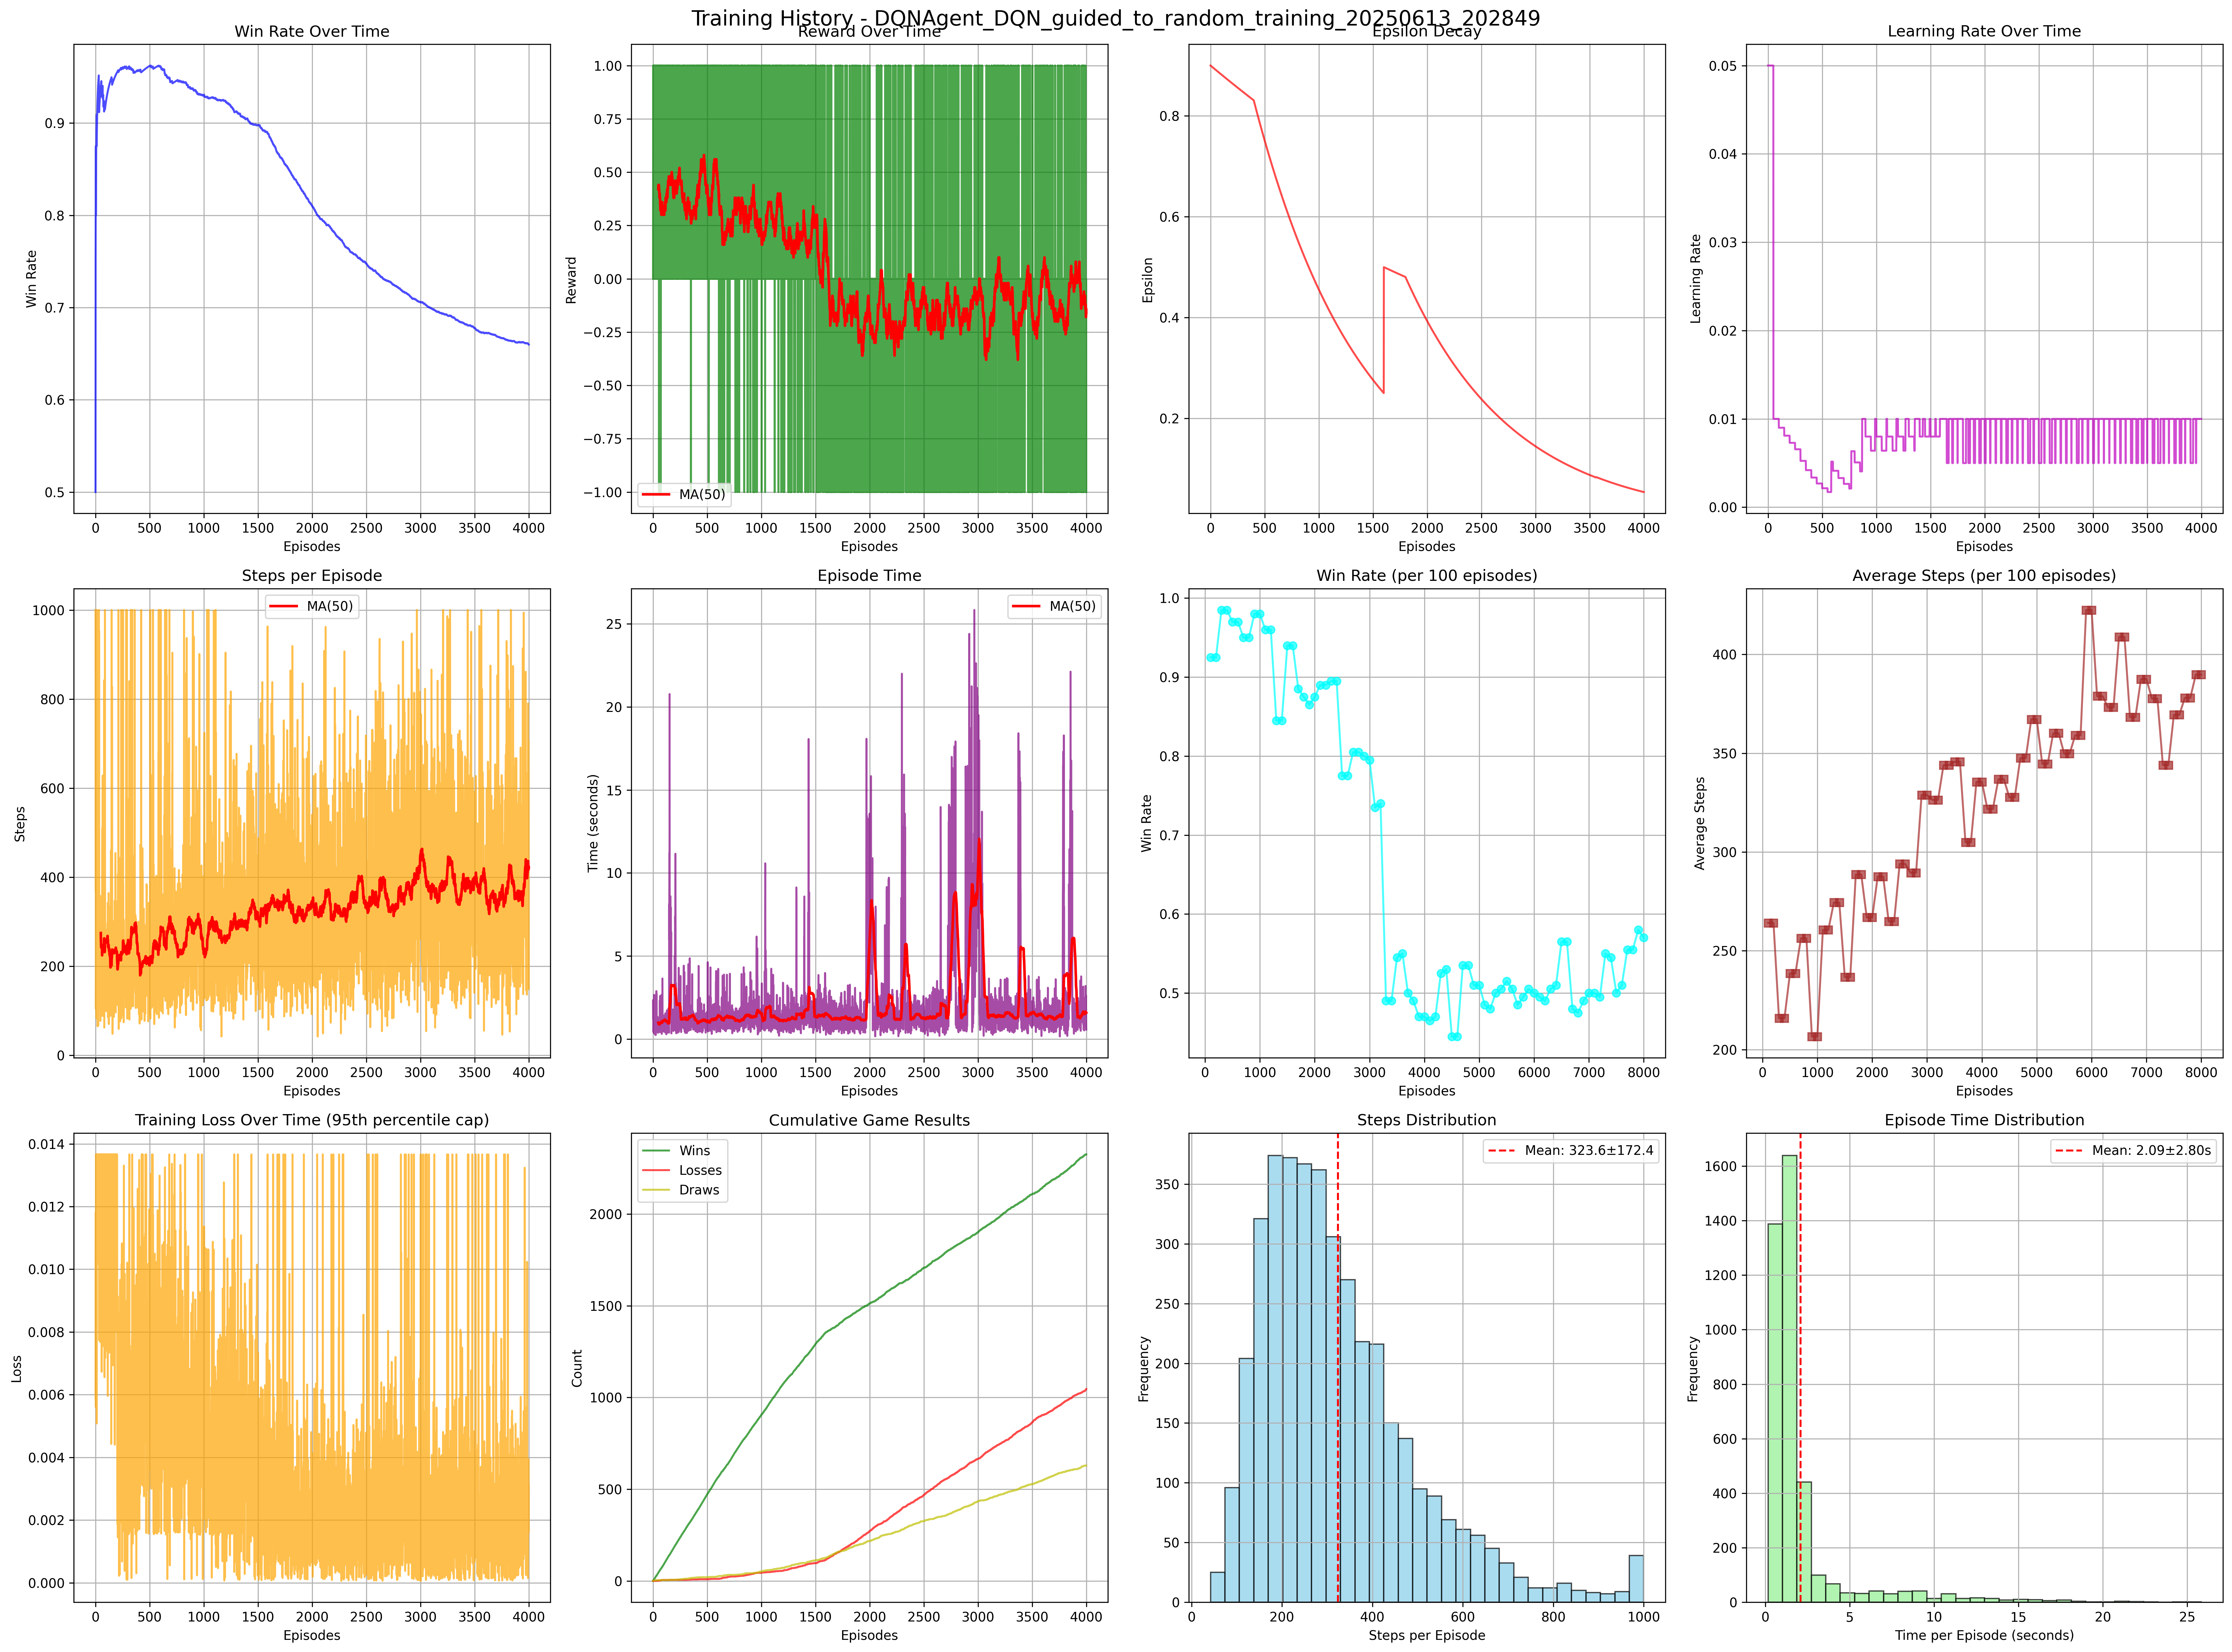
\includegraphics[width=1.0\textwidth]{DQNAgent_training_plots.png}
    \caption{DQN Training Performance}
    \label{fig:dqn_training_curves}
\end{figure}

\subsection{Training Phase Analysis}

\textbf{Phase 1 Analysis (Episodes 1-1,600):} The guided exploration phase shows rapid initial improvement in win rate, reaching approximately 70\% against random opponents. The epsilon decay from 0.9 to 0.02 allows for systematic exploration while leveraging domain knowledge through heuristic guidance.

\textbf{Phase 2 Analysis (Episodes 1,601-4,000):} The transition to random exploration maintains stable performance while allowing for policy refinement. The reduced target network update frequency (1,000 episodes) during this phase promotes learning stability as evidenced by the smoother reward curves.

\textbf{Convergence Characteristics:} The training curves demonstrate successful convergence with minimal overfitting, validating our curriculum learning approach for this complex partial-information game environment.


\subsection{QL and AQ Training Progression}

\begin{figure}[H]
    \centering
    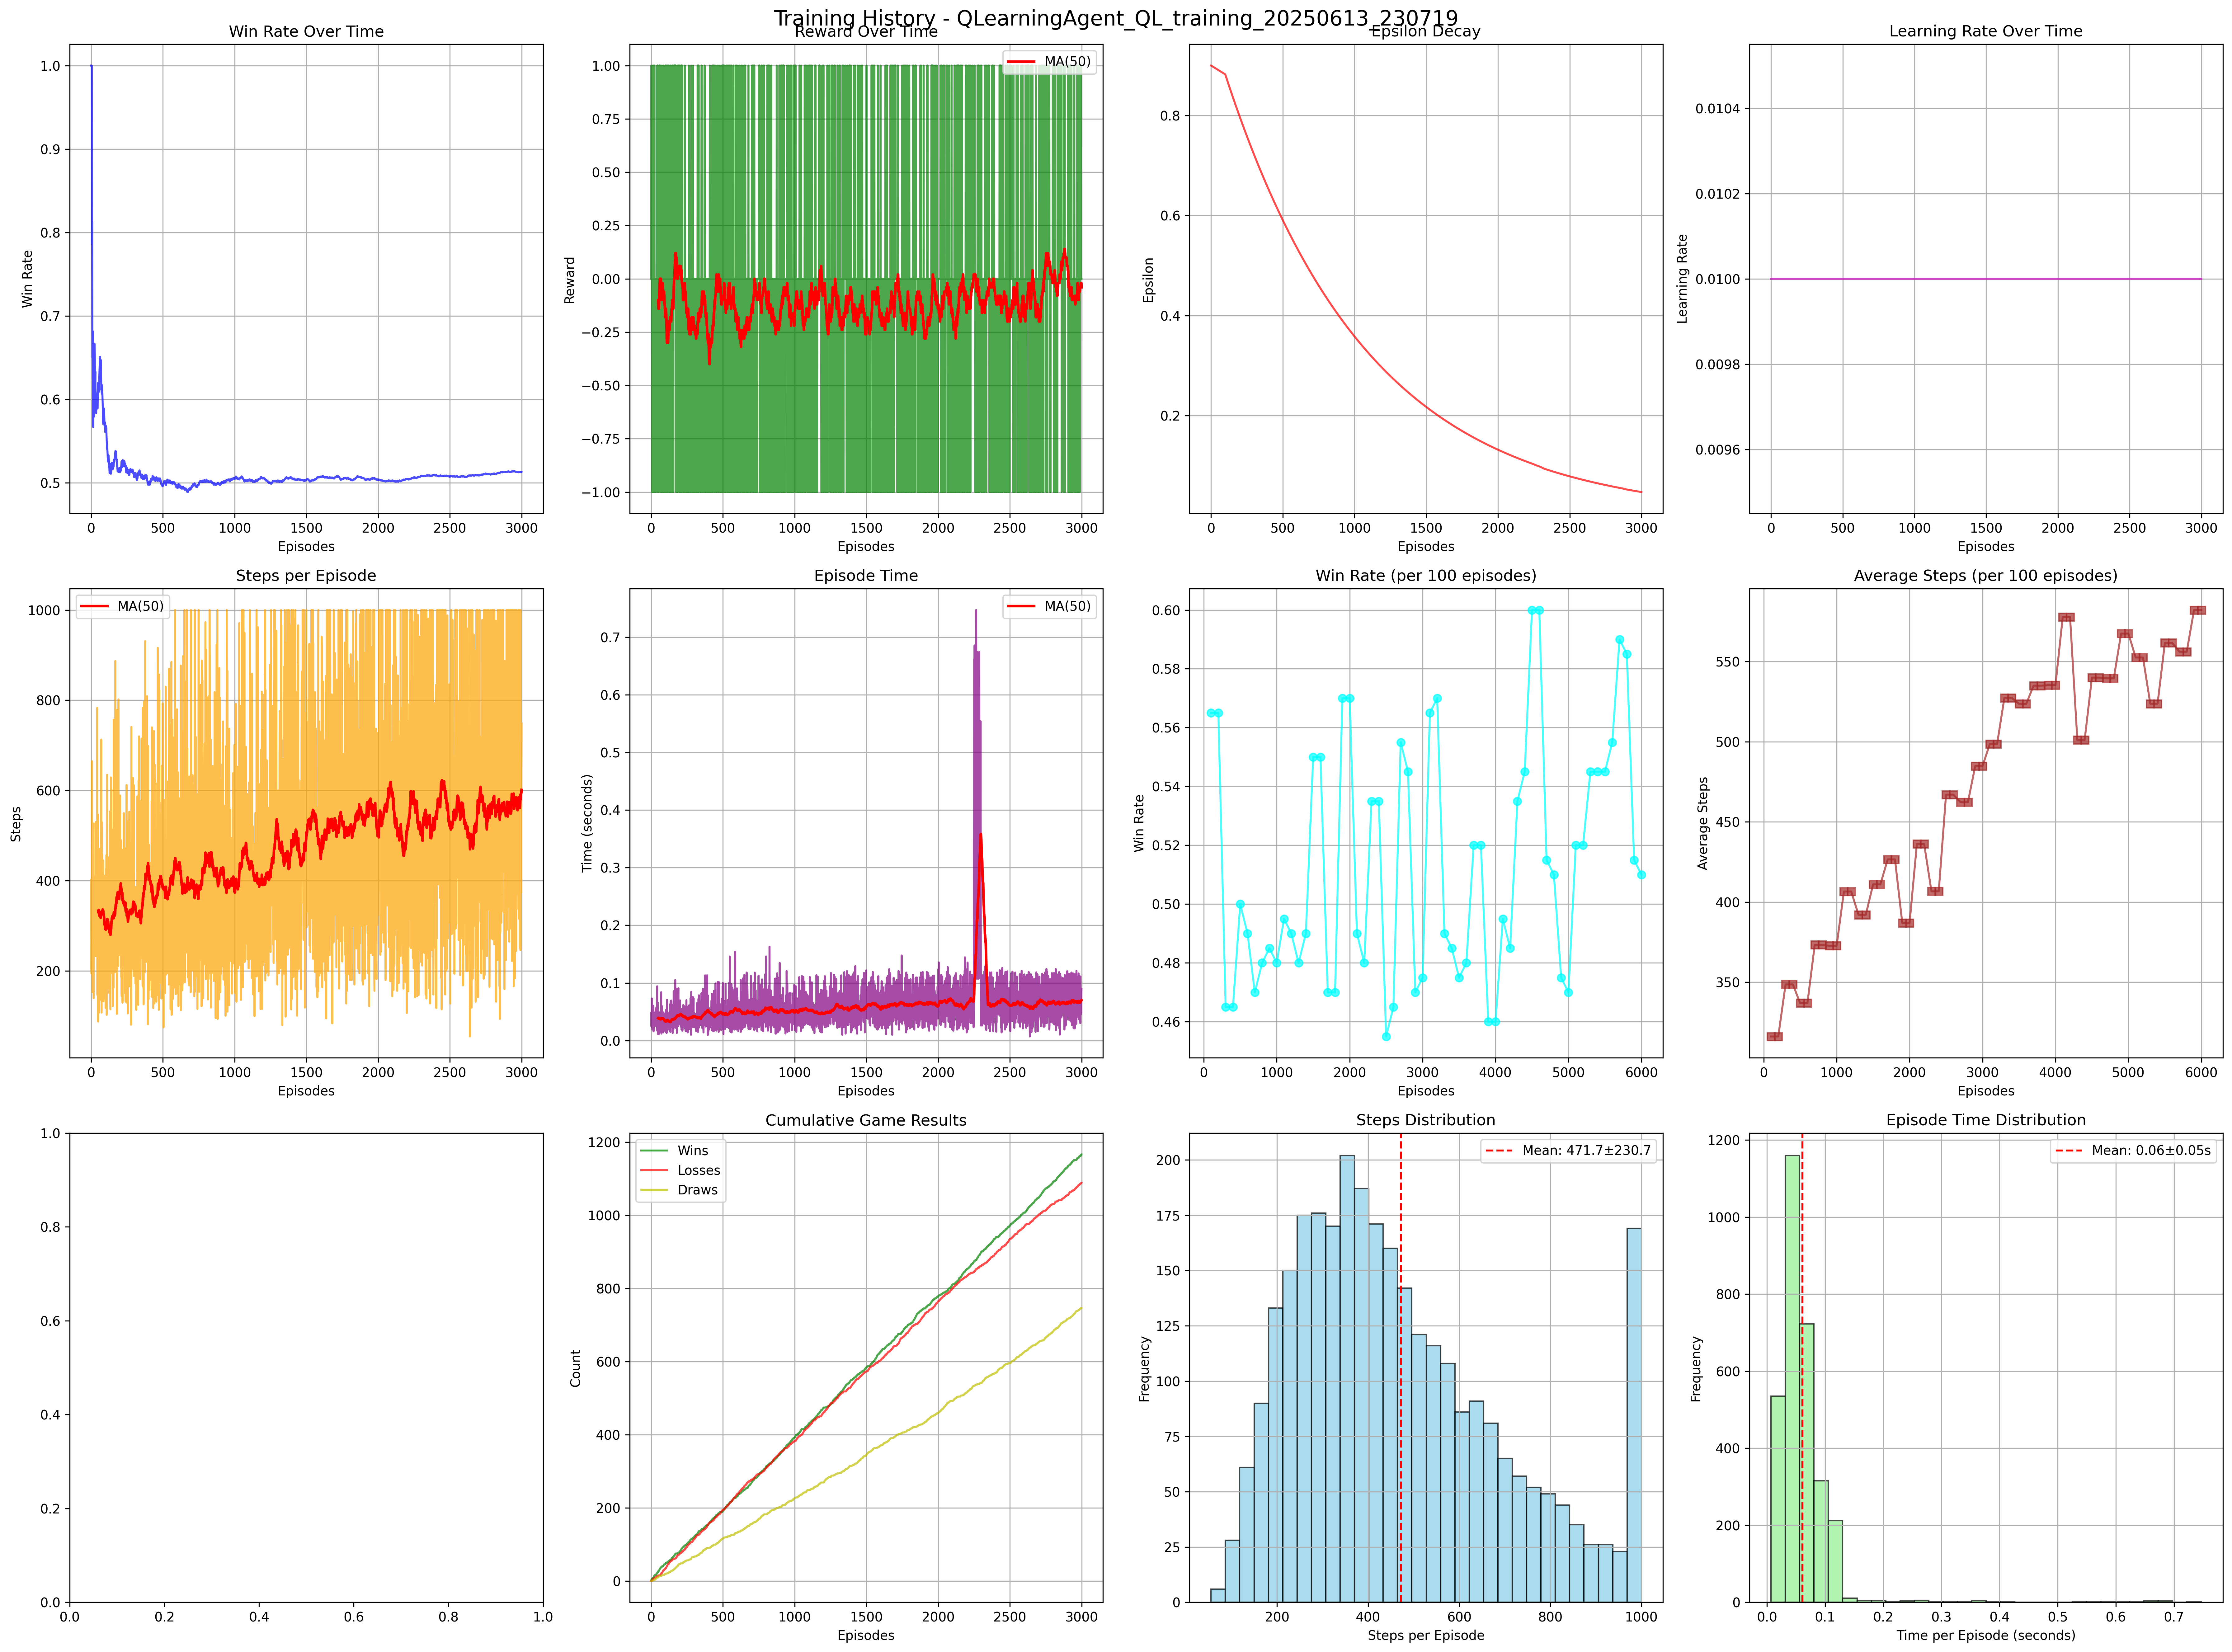
\includegraphics[width=0.9\textwidth]{QLAgent_training_plots.png}
    \caption{QL Training Performance}
    \label{fig:ql_training_curves}
\end{figure}

\begin{figure}[H]
    \centering
    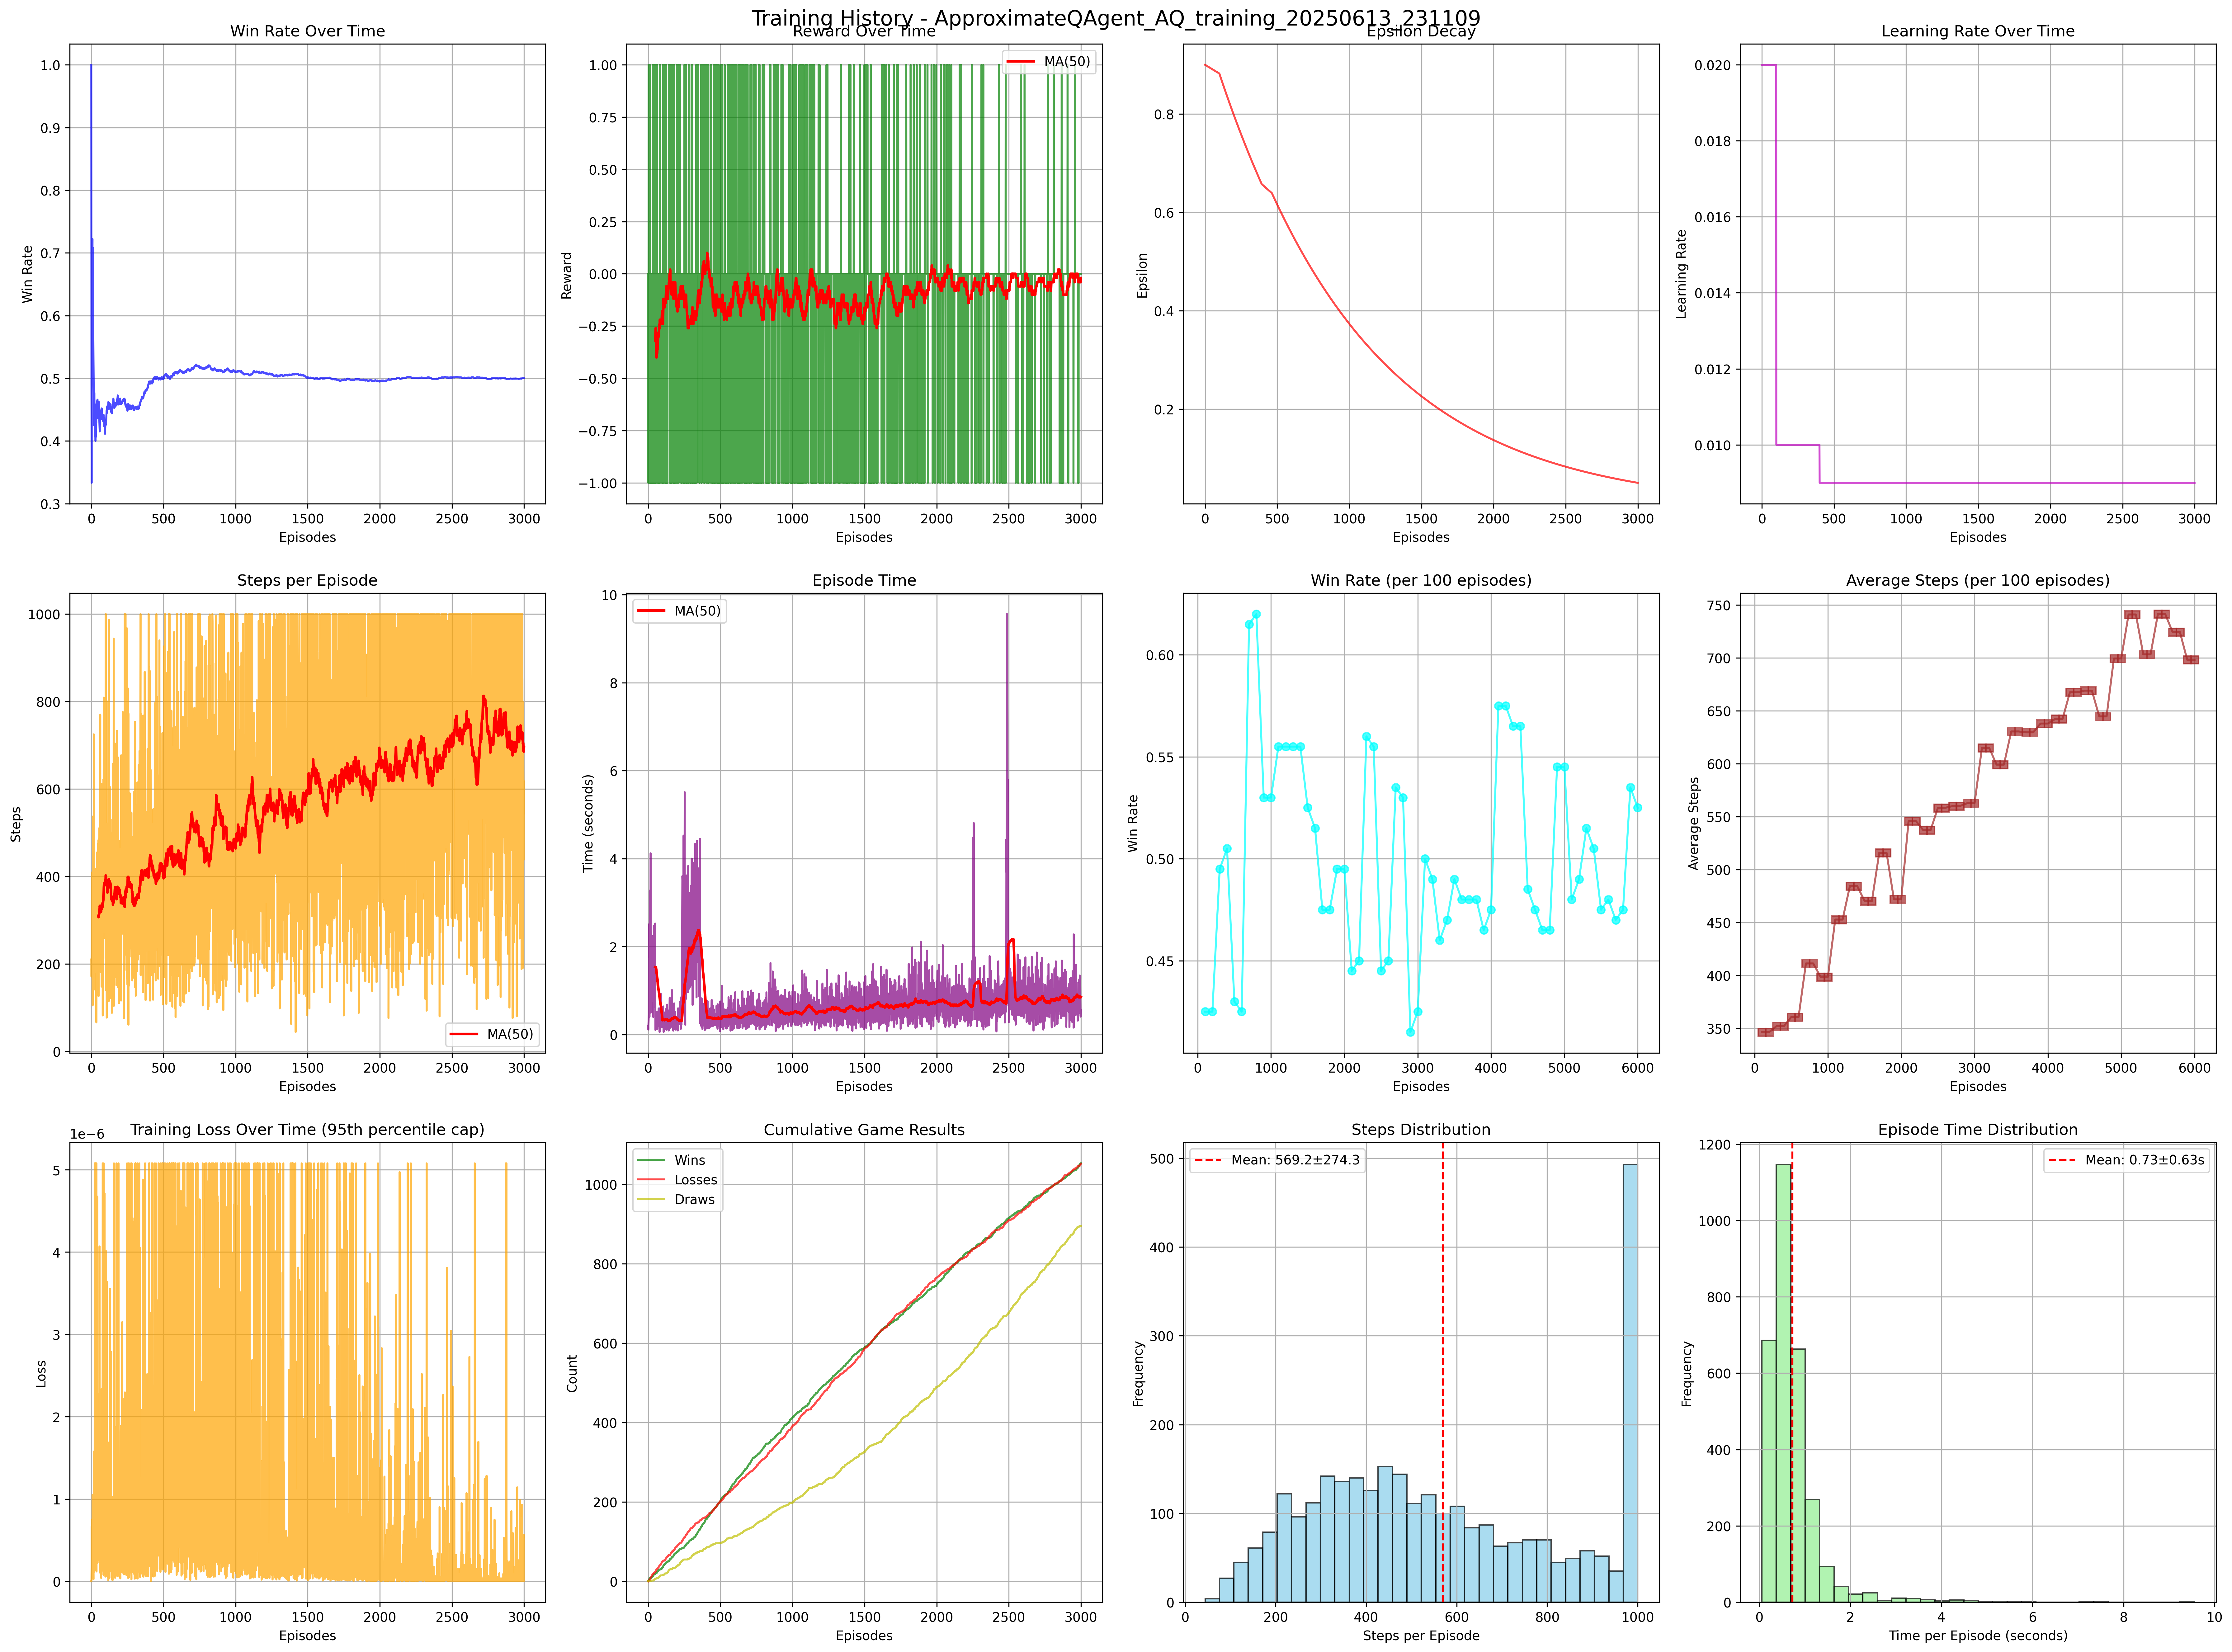
\includegraphics[width=0.9\textwidth]{AQAgent_training_plots.png}
    \caption{AQ Training Performance}
    \label{fig:aq_training_curves}
\end{figure}



\end{document}